%$Header: /home/dashley/cvsrep/e3ft_gpl01/e3ft_gpl01/winprojs/scirfmmon/docs/man20081211a/man20081211a.tex,v 1.20 2009/01/17 22:17:01 dashley Exp $
\documentclass[letterpaper,10pt,titlepage]{article}
//-------------------------------------------------------------------------------------------------
//This source code and any program in which it is compiled/used is provided under the GNU GENERAL
//PUBLIC LICENSE, Version 3, full license text below.
//-------------------------------------------------------------------------------------------------
//                    GNU GENERAL PUBLIC LICENSE
//                       Version 3, 29 June 2007
//
// Copyright (C) 2007 Free Software Foundation, Inc. <http://fsf.org/>
// Everyone is permitted to copy and distribute verbatim copies
// of this license document, but changing it is not allowed.
//
//                            Preamble
//
//  The GNU General Public License is a free, copyleft license for
//software and other kinds of works.
//
//  The licenses for most software and other practical works are designed
//to take away your freedom to share and change the works.  By contrast,
//the GNU General Public License is intended to guarantee your freedom to
//share and change all versions of a program--to make sure it remains free
//software for all its users.  We, the Free Software Foundation, use the
//GNU General Public License for most of our software; it applies also to
//any other work released this way by its authors.  You can apply it to
//your programs, too.
//
//  When we speak of free software, we are referring to freedom, not
//price.  Our General Public Licenses are designed to make sure that you
//have the freedom to distribute copies of free software (and charge for
//them if you wish), that you receive source code or can get it if you
//want it, that you can change the software or use pieces of it in new
//free programs, and that you know you can do these things.
//
//  To protect your rights, we need to prevent others from denying you
//these rights or asking you to surrender the rights.  Therefore, you have
//certain responsibilities if you distribute copies of the software, or if
//you modify it: responsibilities to respect the freedom of others.
//
//  For example, if you distribute copies of such a program, whether
//gratis or for a fee, you must pass on to the recipients the same
//freedoms that you received.  You must make sure that they, too, receive
//or can get the source code.  And you must show them these terms so they
//know their rights.
//
//  Developers that use the GNU GPL protect your rights with two steps:
//(1) assert copyright on the software, and (2) offer you this License
//giving you legal permission to copy, distribute and/or modify it.
//
//  For the developers' and authors' protection, the GPL clearly explains
//that there is no warranty for this free software.  For both users' and
//authors' sake, the GPL requires that modified versions be marked as
//changed, so that their problems will not be attributed erroneously to
//authors of previous versions.
//
//  Some devices are designed to deny users access to install or run
//modified versions of the software inside them, although the manufacturer
//can do so.  This is fundamentally incompatible with the aim of
//protecting users' freedom to change the software.  The systematic
//pattern of such abuse occurs in the area of products for individuals to
//use, which is precisely where it is most unacceptable.  Therefore, we
//have designed this version of the GPL to prohibit the practice for those
//products.  If such problems arise substantially in other domains, we
//stand ready to extend this provision to those domains in future versions
//of the GPL, as needed to protect the freedom of users.
//
//  Finally, every program is threatened constantly by software patents.
//States should not allow patents to restrict development and use of
//software on general-purpose computers, but in those that do, we wish to
//avoid the special danger that patents applied to a free program could
//make it effectively proprietary.  To prevent this, the GPL assures that
//patents cannot be used to render the program non-free.
//
//  The precise terms and conditions for copying, distribution and
//modification follow.
//
//                       TERMS AND CONDITIONS
//
//  0. Definitions.
//
//  "This License" refers to version 3 of the GNU General Public License.
//
//  "Copyright" also means copyright-like laws that apply to other kinds of
//works, such as semiconductor masks.
//
//  "The Program" refers to any copyrightable work licensed under this
//License.  Each licensee is addressed as "you".  "Licensees" and
//"recipients" may be individuals or organizations.
//
//  To "modify" a work means to copy from or adapt all or part of the work
//in a fashion requiring copyright permission, other than the making of an
//exact copy.  The resulting work is called a "modified version" of the
//earlier work or a work "based on" the earlier work.
//
//  A "covered work" means either the unmodified Program or a work based
//on the Program.
//
//  To "propagate" a work means to do anything with it that, without
//permission, would make you directly or secondarily liable for
//infringement under applicable copyright law, except executing it on a
//computer or modifying a private copy.  Propagation includes copying,
//distribution (with or without modification), making available to the
//public, and in some countries other activities as well.
//
//  To "convey" a work means any kind of propagation that enables other
//parties to make or receive copies.  Mere interaction with a user through
//a computer network, with no transfer of a copy, is not conveying.
//
//  An interactive user interface displays "Appropriate Legal Notices"
//to the extent that it includes a convenient and prominently visible
//feature that (1) displays an appropriate copyright notice, and (2)
//tells the user that there is no warranty for the work (except to the
//extent that warranties are provided), that licensees may convey the
//work under this License, and how to view a copy of this License.  If
//the interface presents a list of user commands or options, such as a
//menu, a prominent item in the list meets this criterion.
//
//  1. Source Code.
//
//  The "source code" for a work means the preferred form of the work
//for making modifications to it.  "Object code" means any non-source
//form of a work.
//
//  A "Standard Interface" means an interface that either is an official
//standard defined by a recognized standards body, or, in the case of
//interfaces specified for a particular programming language, one that
//is widely used among developers working in that language.
//
//  The "System Libraries" of an executable work include anything, other
//than the work as a whole, that (a) is included in the normal form of
//packaging a Major Component, but which is not part of that Major
//Component, and (b) serves only to enable use of the work with that
//Major Component, or to implement a Standard Interface for which an
//implementation is available to the public in source code form.  A
//"Major Component", in this context, means a major essential component
//(kernel, window system, and so on) of the specific operating system
//(if any) on which the executable work runs, or a compiler used to
//produce the work, or an object code interpreter used to run it.
//
//  The "Corresponding Source" for a work in object code form means all
//the source code needed to generate, install, and (for an executable
//work) run the object code and to modify the work, including scripts to
//control those activities.  However, it does not include the work's
//System Libraries, or general-purpose tools or generally available free
//programs which are used unmodified in performing those activities but
//which are not part of the work.  For example, Corresponding Source
//includes interface definition files associated with source files for
//the work, and the source code for shared libraries and dynamically
//linked subprograms that the work is specifically designed to require,
//such as by intimate data communication or control flow between those
//subprograms and other parts of the work.
//
//  The Corresponding Source need not include anything that users
//can regenerate automatically from other parts of the Corresponding
//Source.
//
//  The Corresponding Source for a work in source code form is that
//same work.
//
//  2. Basic Permissions.
//
//  All rights granted under this License are granted for the term of
//copyright on the Program, and are irrevocable provided the stated
//conditions are met.  This License explicitly affirms your unlimited
//permission to run the unmodified Program.  The output from running a
//covered work is covered by this License only if the output, given its
//content, constitutes a covered work.  This License acknowledges your
//rights of fair use or other equivalent, as provided by copyright law.
//
//  You may make, run and propagate covered works that you do not
//convey, without conditions so long as your license otherwise remains
//in force.  You may convey covered works to others for the sole purpose
//of having them make modifications exclusively for you, or provide you
//with facilities for running those works, provided that you comply with
//the terms of this License in conveying all material for which you do
//not control copyright.  Those thus making or running the covered works
//for you must do so exclusively on your behalf, under your direction
//and control, on terms that prohibit them from making any copies of
//your copyrighted material outside their relationship with you.
//
//  Conveying under any other circumstances is permitted solely under
//the conditions stated below.  Sublicensing is not allowed; section 10
//makes it unnecessary.
//
//  3. Protecting Users' Legal Rights From Anti-Circumvention Law.
//
//  No covered work shall be deemed part of an effective technological
//measure under any applicable law fulfilling obligations under article
//11 of the WIPO copyright treaty adopted on 20 December 1996, or
//similar laws prohibiting or restricting circumvention of such
//measures.
//
//  When you convey a covered work, you waive any legal power to forbid
//circumvention of technological measures to the extent such circumvention
//is effected by exercising rights under this License with respect to
//the covered work, and you disclaim any intention to limit operation or
//modification of the work as a means of enforcing, against the work's
//users, your or third parties' legal rights to forbid circumvention of
//technological measures.
//
//  4. Conveying Verbatim Copies.
//
//  You may convey verbatim copies of the Program's source code as you
//receive it, in any medium, provided that you conspicuously and
//appropriately publish on each copy an appropriate copyright notice;
//keep intact all notices stating that this License and any
//non-permissive terms added in accord with section 7 apply to the code;
//keep intact all notices of the absence of any warranty; and give all
//recipients a copy of this License along with the Program.
//
//  You may charge any price or no price for each copy that you convey,
//and you may offer support or warranty protection for a fee.
//
//  5. Conveying Modified Source Versions.
//
//  You may convey a work based on the Program, or the modifications to
//produce it from the Program, in the form of source code under the
//terms of section 4, provided that you also meet all of these conditions:
//
//    a) The work must carry prominent notices stating that you modified
//    it, and giving a relevant date.
//
//    b) The work must carry prominent notices stating that it is
//    released under this License and any conditions added under section
//    7.  This requirement modifies the requirement in section 4 to
//    "keep intact all notices".
//
//    c) You must license the entire work, as a whole, under this
//    License to anyone who comes into possession of a copy.  This
//    License will therefore apply, along with any applicable section 7
//    additional terms, to the whole of the work, and all its parts,
//    regardless of how they are packaged.  This License gives no
//    permission to license the work in any other way, but it does not
//    invalidate such permission if you have separately received it.
//
//    d) If the work has interactive user interfaces, each must display
//    Appropriate Legal Notices; however, if the Program has interactive
//    interfaces that do not display Appropriate Legal Notices, your
//    work need not make them do so.
//
//  A compilation of a covered work with other separate and independent
//works, which are not by their nature extensions of the covered work,
//and which are not combined with it such as to form a larger program,
//in or on a volume of a storage or distribution medium, is called an
//"aggregate" if the compilation and its resulting copyright are not
//used to limit the access or legal rights of the compilation's users
//beyond what the individual works permit.  Inclusion of a covered work
//in an aggregate does not cause this License to apply to the other
//parts of the aggregate.
//
//  6. Conveying Non-Source Forms.
//
//  You may convey a covered work in object code form under the terms
//of sections 4 and 5, provided that you also convey the
//machine-readable Corresponding Source under the terms of this License,
//in one of these ways:
//
//    a) Convey the object code in, or embodied in, a physical product
//    (including a physical distribution medium), accompanied by the
//    Corresponding Source fixed on a durable physical medium
//    customarily used for software interchange.
//
//    b) Convey the object code in, or embodied in, a physical product
//    (including a physical distribution medium), accompanied by a
//    written offer, valid for at least three years and valid for as
//    long as you offer spare parts or customer support for that product
//    model, to give anyone who possesses the object code either (1) a
//    copy of the Corresponding Source for all the software in the
//    product that is covered by this License, on a durable physical
//    medium customarily used for software interchange, for a price no
//    more than your reasonable cost of physically performing this
//    conveying of source, or (2) access to copy the
//    Corresponding Source from a network server at no charge.
//
//    c) Convey individual copies of the object code with a copy of the
//    written offer to provide the Corresponding Source.  This
//    alternative is allowed only occasionally and noncommercially, and
//    only if you received the object code with such an offer, in accord
//    with subsection 6b.
//
//    d) Convey the object code by offering access from a designated
//    place (gratis or for a charge), and offer equivalent access to the
//    Corresponding Source in the same way through the same place at no
//    further charge.  You need not require recipients to copy the
//    Corresponding Source along with the object code.  If the place to
//    copy the object code is a network server, the Corresponding Source
//    may be on a different server (operated by you or a third party)
//    that supports equivalent copying facilities, provided you maintain
//    clear directions next to the object code saying where to find the
//    Corresponding Source.  Regardless of what server hosts the
//    Corresponding Source, you remain obligated to ensure that it is
//    available for as long as needed to satisfy these requirements.
//
//    e) Convey the object code using peer-to-peer transmission, provided
//    you inform other peers where the object code and Corresponding
//    Source of the work are being offered to the general public at no
//    charge under subsection 6d.
//
//  A separable portion of the object code, whose source code is excluded
//from the Corresponding Source as a System Library, need not be
//included in conveying the object code work.
//
//  A "User Product" is either (1) a "consumer product", which means any
//tangible personal property which is normally used for personal, family,
//or household purposes, or (2) anything designed or sold for incorporation
//into a dwelling.  In determining whether a product is a consumer product,
//doubtful cases shall be resolved in favor of coverage.  For a particular
//product received by a particular user, "normally used" refers to a
//typical or common use of that class of product, regardless of the status
//of the particular user or of the way in which the particular user
//actually uses, or expects or is expected to use, the product.  A product
//is a consumer product regardless of whether the product has substantial
//commercial, industrial or non-consumer uses, unless such uses represent
//the only significant mode of use of the product.
//
//  "Installation Information" for a User Product means any methods,
//procedures, authorization keys, or other information required to install
//and execute modified versions of a covered work in that User Product from
//a modified version of its Corresponding Source.  The information must
//suffice to ensure that the continued functioning of the modified object
//code is in no case prevented or interfered with solely because
//modification has been made.
//
//  If you convey an object code work under this section in, or with, or
//specifically for use in, a User Product, and the conveying occurs as
//part of a transaction in which the right of possession and use of the
//User Product is transferred to the recipient in perpetuity or for a
//fixed term (regardless of how the transaction is characterized), the
//Corresponding Source conveyed under this section must be accompanied
//by the Installation Information.  But this requirement does not apply
//if neither you nor any third party retains the ability to install
//modified object code on the User Product (for example, the work has
//been installed in ROM).
//
//  The requirement to provide Installation Information does not include a
//requirement to continue to provide support service, warranty, or updates
//for a work that has been modified or installed by the recipient, or for
//the User Product in which it has been modified or installed.  Access to a
//network may be denied when the modification itself materially and
//adversely affects the operation of the network or violates the rules and
//protocols for communication across the network.
//
//  Corresponding Source conveyed, and Installation Information provided,
//in accord with this section must be in a format that is publicly
//documented (and with an implementation available to the public in
//source code form), and must require no special password or key for
//unpacking, reading or copying.
//
//  7. Additional Terms.
//
//  "Additional permissions" are terms that supplement the terms of this
//License by making exceptions from one or more of its conditions.
//Additional permissions that are applicable to the entire Program shall
//be treated as though they were included in this License, to the extent
//that they are valid under applicable law.  If additional permissions
//apply only to part of the Program, that part may be used separately
//under those permissions, but the entire Program remains governed by
//this License without regard to the additional permissions.
//
//  When you convey a copy of a covered work, you may at your option
//remove any additional permissions from that copy, or from any part of
//it.  (Additional permissions may be written to require their own
//removal in certain cases when you modify the work.)  You may place
//additional permissions on material, added by you to a covered work,
//for which you have or can give appropriate copyright permission.
//
//  Notwithstanding any other provision of this License, for material you
//add to a covered work, you may (if authorized by the copyright holders of
//that material) supplement the terms of this License with terms:
//
//    a) Disclaiming warranty or limiting liability differently from the
//    terms of sections 15 and 16 of this License; or
//
//    b) Requiring preservation of specified reasonable legal notices or
//    author attributions in that material or in the Appropriate Legal
//    Notices displayed by works containing it; or
//
//    c) Prohibiting misrepresentation of the origin of that material, or
//    requiring that modified versions of such material be marked in
//    reasonable ways as different from the original version; or
//
//    d) Limiting the use for publicity purposes of names of licensors or
//    authors of the material; or
//
//    e) Declining to grant rights under trademark law for use of some
//    trade names, trademarks, or service marks; or
//
//    f) Requiring indemnification of licensors and authors of that
//    material by anyone who conveys the material (or modified versions of
//    it) with contractual assumptions of liability to the recipient, for
//    any liability that these contractual assumptions directly impose on
//    those licensors and authors.
//
//  All other non-permissive additional terms are considered "further
//restrictions" within the meaning of section 10.  If the Program as you
//received it, or any part of it, contains a notice stating that it is
//governed by this License along with a term that is a further
//restriction, you may remove that term.  If a license document contains
//a further restriction but permits relicensing or conveying under this
//License, you may add to a covered work material governed by the terms
//of that license document, provided that the further restriction does
//not survive such relicensing or conveying.
//
//  If you add terms to a covered work in accord with this section, you
//must place, in the relevant source files, a statement of the
//additional terms that apply to those files, or a notice indicating
//where to find the applicable terms.
//
//  Additional terms, permissive or non-permissive, may be stated in the
//form of a separately written license, or stated as exceptions;
//the above requirements apply either way.
//
//  8. Termination.
//
//  You may not propagate or modify a covered work except as expressly
//provided under this License.  Any attempt otherwise to propagate or
//modify it is void, and will automatically terminate your rights under
//this License (including any patent licenses granted under the third
//paragraph of section 11).
//
//  However, if you cease all violation of this License, then your
//license from a particular copyright holder is reinstated (a)
//provisionally, unless and until the copyright holder explicitly and
//finally terminates your license, and (b) permanently, if the copyright
//holder fails to notify you of the violation by some reasonable means
//prior to 60 days after the cessation.
//
//  Moreover, your license from a particular copyright holder is
//reinstated permanently if the copyright holder notifies you of the
//violation by some reasonable means, this is the first time you have
//received notice of violation of this License (for any work) from that
//copyright holder, and you cure the violation prior to 30 days after
//your receipt of the notice.
//
//  Termination of your rights under this section does not terminate the
//licenses of parties who have received copies or rights from you under
//this License.  If your rights have been terminated and not permanently
//reinstated, you do not qualify to receive new licenses for the same
//material under section 10.
//
//  9. Acceptance Not Required for Having Copies.
//
//  You are not required to accept this License in order to receive or
//run a copy of the Program.  Ancillary propagation of a covered work
//occurring solely as a consequence of using peer-to-peer transmission
//to receive a copy likewise does not require acceptance.  However,
//nothing other than this License grants you permission to propagate or
//modify any covered work.  These actions infringe copyright if you do
//not accept this License.  Therefore, by modifying or propagating a
//covered work, you indicate your acceptance of this License to do so.
//
//  10. Automatic Licensing of Downstream Recipients.
//
//  Each time you convey a covered work, the recipient automatically
//receives a license from the original licensors, to run, modify and
//propagate that work, subject to this License.  You are not responsible
//for enforcing compliance by third parties with this License.
//
//  An "entity transaction" is a transaction transferring control of an
//organization, or substantially all assets of one, or subdividing an
//organization, or merging organizations.  If propagation of a covered
//work results from an entity transaction, each party to that
//transaction who receives a copy of the work also receives whatever
//licenses to the work the party's predecessor in interest had or could
//give under the previous paragraph, plus a right to possession of the
//Corresponding Source of the work from the predecessor in interest, if
//the predecessor has it or can get it with reasonable efforts.
//
//  You may not impose any further restrictions on the exercise of the
//rights granted or affirmed under this License.  For example, you may
//not impose a license fee, royalty, or other charge for exercise of
//rights granted under this License, and you may not initiate litigation
//(including a cross-claim or counterclaim in a lawsuit) alleging that
//any patent claim is infringed by making, using, selling, offering for
//sale, or importing the Program or any portion of it.
//
//  11. Patents.
//
//  A "contributor" is a copyright holder who authorizes use under this
//License of the Program or a work on which the Program is based.  The
//work thus licensed is called the contributor's "contributor version".
//
//  A contributor's "essential patent claims" are all patent claims
//owned or controlled by the contributor, whether already acquired or
//hereafter acquired, that would be infringed by some manner, permitted
//by this License, of making, using, or selling its contributor version,
//but do not include claims that would be infringed only as a
//consequence of further modification of the contributor version.  For
//purposes of this definition, "control" includes the right to grant
//patent sublicenses in a manner consistent with the requirements of
//this License.
//
//  Each contributor grants you a non-exclusive, worldwide, royalty-free
//patent license under the contributor's essential patent claims, to
//make, use, sell, offer for sale, import and otherwise run, modify and
//propagate the contents of its contributor version.
//
//  In the following three paragraphs, a "patent license" is any express
//agreement or commitment, however denominated, not to enforce a patent
//(such as an express permission to practice a patent or covenant not to
//sue for patent infringement).  To "grant" such a patent license to a
//party means to make such an agreement or commitment not to enforce a
//patent against the party.
//
//  If you convey a covered work, knowingly relying on a patent license,
//and the Corresponding Source of the work is not available for anyone
//to copy, free of charge and under the terms of this License, through a
//publicly available network server or other readily accessible means,
//then you must either (1) cause the Corresponding Source to be so
//available, or (2) arrange to deprive yourself of the benefit of the
//patent license for this particular work, or (3) arrange, in a manner
//consistent with the requirements of this License, to extend the patent
//license to downstream recipients.  "Knowingly relying" means you have
//actual knowledge that, but for the patent license, your conveying the
//covered work in a country, or your recipient's use of the covered work
//in a country, would infringe one or more identifiable patents in that
//country that you have reason to believe are valid.
//
//  If, pursuant to or in connection with a single transaction or
//arrangement, you convey, or propagate by procuring conveyance of, a
//covered work, and grant a patent license to some of the parties
//receiving the covered work authorizing them to use, propagate, modify
//or convey a specific copy of the covered work, then the patent license
//you grant is automatically extended to all recipients of the covered
//work and works based on it.
//
//  A patent license is "discriminatory" if it does not include within
//the scope of its coverage, prohibits the exercise of, or is
//conditioned on the non-exercise of one or more of the rights that are
//specifically granted under this License.  You may not convey a covered
//work if you are a party to an arrangement with a third party that is
//in the business of distributing software, under which you make payment
//to the third party based on the extent of your activity of conveying
//the work, and under which the third party grants, to any of the
//parties who would receive the covered work from you, a discriminatory
//patent license (a) in connection with copies of the covered work
//conveyed by you (or copies made from those copies), or (b) primarily
//for and in connection with specific products or compilations that
//contain the covered work, unless you entered into that arrangement,
//or that patent license was granted, prior to 28 March 2007.
//
//  Nothing in this License shall be construed as excluding or limiting
//any implied license or other defenses to infringement that may
//otherwise be available to you under applicable patent law.
//
//  12. No Surrender of Others' Freedom.
//
//  If conditions are imposed on you (whether by court order, agreement or
//otherwise) that contradict the conditions of this License, they do not
//excuse you from the conditions of this License.  If you cannot convey a
//covered work so as to satisfy simultaneously your obligations under this
//License and any other pertinent obligations, then as a consequence you may
//not convey it at all.  For example, if you agree to terms that obligate you
//to collect a royalty for further conveying from those to whom you convey
//the Program, the only way you could satisfy both those terms and this
//License would be to refrain entirely from conveying the Program.
//
//  13. Use with the GNU Affero General Public License.
//
//  Notwithstanding any other provision of this License, you have
//permission to link or combine any covered work with a work licensed
//under version 3 of the GNU Affero General Public License into a single
//combined work, and to convey the resulting work.  The terms of this
//License will continue to apply to the part which is the covered work,
//but the special requirements of the GNU Affero General Public License,
//section 13, concerning interaction through a network will apply to the
//combination as such.
//
//  14. Revised Versions of this License.
//
//  The Free Software Foundation may publish revised and/or new versions of
//the GNU General Public License from time to time.  Such new versions will
//be similar in spirit to the present version, but may differ in detail to
//address new problems or concerns.
//
//  Each version is given a distinguishing version number.  If the
//Program specifies that a certain numbered version of the GNU General
//Public License "or any later version" applies to it, you have the
//option of following the terms and conditions either of that numbered
//version or of any later version published by the Free Software
//Foundation.  If the Program does not specify a version number of the
//GNU General Public License, you may choose any version ever published
//by the Free Software Foundation.
//
//  If the Program specifies that a proxy can decide which future
//versions of the GNU General Public License can be used, that proxy's
//public statement of acceptance of a version permanently authorizes you
//to choose that version for the Program.
//
//  Later license versions may give you additional or different
//permissions.  However, no additional obligations are imposed on any
//author or copyright holder as a result of your choosing to follow a
//later version.
//
//  15. Disclaimer of Warranty.
//
//  THERE IS NO WARRANTY FOR THE PROGRAM, TO THE EXTENT PERMITTED BY
//APPLICABLE LAW.  EXCEPT WHEN OTHERWISE STATED IN WRITING THE COPYRIGHT
//HOLDERS AND/OR OTHER PARTIES PROVIDE THE PROGRAM "AS IS" WITHOUT WARRANTY
//OF ANY KIND, EITHER EXPRESSED OR IMPLIED, INCLUDING, BUT NOT LIMITED TO,
//THE IMPLIED WARRANTIES OF MERCHANTABILITY AND FITNESS FOR A PARTICULAR
//PURPOSE.  THE ENTIRE RISK AS TO THE QUALITY AND PERFORMANCE OF THE PROGRAM
//IS WITH YOU.  SHOULD THE PROGRAM PROVE DEFECTIVE, YOU ASSUME THE COST OF
//ALL NECESSARY SERVICING, REPAIR OR CORRECTION.
//
//  16. Limitation of Liability.
//
//  IN NO EVENT UNLESS REQUIRED BY APPLICABLE LAW OR AGREED TO IN WRITING
//WILL ANY COPYRIGHT HOLDER, OR ANY OTHER PARTY WHO MODIFIES AND/OR CONVEYS
//THE PROGRAM AS PERMITTED ABOVE, BE LIABLE TO YOU FOR DAMAGES, INCLUDING ANY
//GENERAL, SPECIAL, INCIDENTAL OR CONSEQUENTIAL DAMAGES ARISING OUT OF THE
//USE OR INABILITY TO USE THE PROGRAM (INCLUDING BUT NOT LIMITED TO LOSS OF
//DATA OR DATA BEING RENDERED INACCURATE OR LOSSES SUSTAINED BY YOU OR THIRD
//PARTIES OR A FAILURE OF THE PROGRAM TO OPERATE WITH ANY OTHER PROGRAMS),
//EVEN IF SUCH HOLDER OR OTHER PARTY HAS BEEN ADVISED OF THE POSSIBILITY OF
//SUCH DAMAGES.
//
//  17. Interpretation of Sections 15 and 16.
//
//  If the disclaimer of warranty and limitation of liability provided
//above cannot be given local legal effect according to their terms,
//reviewing courts shall apply local law that most closely approximates
//an absolute waiver of all civil liability in connection with the
//Program, unless a warranty or assumption of liability accompanies a
//copy of the Program in return for a fee.
//
//                     END OF TERMS AND CONDITIONS
//
//            How to Apply These Terms to Your New Programs
//
//  If you develop a new program, and you want it to be of the greatest
//possible use to the public, the best way to achieve this is to make it
//free software which everyone can redistribute and change under these terms.
//
//  To do so, attach the following notices to the program.  It is safest
//to attach them to the start of each source file to most effectively
//state the exclusion of warranty; and each file should have at least
//the "copyright" line and a pointer to where the full notice is found.
//
//    <one line to give the program's name and a brief idea of what it does.>
//    Copyright (C) <year>  <name of author>
//
//    This program is free software: you can redistribute it and/or modify
//    it under the terms of the GNU General Public License as published by
//    the Free Software Foundation, either version 3 of the License, or
//    (at your option) any later version.
//
//    This program is distributed in the hope that it will be useful,
//    but WITHOUT ANY WARRANTY; without even the implied warranty of
//    MERCHANTABILITY or FITNESS FOR A PARTICULAR PURPOSE.  See the
//    GNU General Public License for more details.
//
//    You should have received a copy of the GNU General Public License
//    along with this program.  If not, see <http://www.gnu.org/licenses/>.
//
//Also add information on how to contact you by electronic and paper mail.
//
//  If the program does terminal interaction, make it output a short
//notice like this when it starts in an interactive mode:
//
//    <program>  Copyright (C) <year>  <name of author>
//    This program comes with ABSOLUTELY NO WARRANTY; for details type `show w'.
//    This is free software, and you are welcome to redistribute it
//    under certain conditions; type `show c' for details.
//
//The hypothetical commands `show w' and `show c' should show the appropriate
//parts of the General Public License.  Of course, your program's commands
//might be different; for a GUI interface, you would use an "about box".
//
//  You should also get your employer (if you work as a programmer) or school,
//if any, to sign a "copyright disclaimer" for the program, if necessary.
//For more information on this, and how to apply and follow the GNU GPL, see
//<http://www.gnu.org/licenses/>.
//
//  The GNU General Public License does not permit incorporating your program
//into proprietary programs.  If your program is a subroutine library, you
//may consider it more useful to permit linking proprietary applications with
//the library.  If this is what you want to do, use the GNU Lesser General
//Public License instead of this License.  But first, please read
//<http://www.gnu.org/philosophy/why-not-lgpl.html>.
//-------------------------------------------------------------------------------------------------%
%\pagestyle{headings}
%
\usepackage{amsmath}
\usepackage{amsfonts}
\usepackage{amssymb}
\usepackage[ansinew]{inputenc}
\usepackage[OT1]{fontenc}
\usepackage{graphicx}
\usepackage{makeidx}
%
%-----------------------------------------------------------------------------------
%Constants
\newcommand{\productversion}{0.1a}
\newcommand{\productname}{scirfmmon}
\newcommand{\productnameemph}{\emph{\productname}}
\newcommand{\productcompiledate}{Jan 17 2009}
\newcommand{\productassertletter}{a}
\newcommand{\productversionhash}{63570560d4fd6dc71431d7bca67c8ff35c9fd1fe}
%-----------------------------------------------------------------------------------
%New environments
%The following environment is for the glossary of terms at the end, if
%included.
\newenvironment{docglossaryenum}{\begin{list}
               {}{\setlength{\labelwidth}{0mm}
                  \setlength{\leftmargin}{4mm}
                  \setlength{\itemindent}{-4mm}
                  \setlength{\parsep}{0.85mm}}}
               {\end{list}}
%%
%The following environment is for the database table and field
%documentation at the end, if included.
\newenvironment{docdbtblfielddef}{\begin{list}
               {}{\setlength{\labelwidth}{0mm}
                  \setlength{\leftmargin}{10mm}
                  \setlength{\itemindent}{-5mm}
                  \setlength{\parsep}{0.85mm}}}
               {\end{list}}
%%
%-----------------------------------------------------------------------------------
%Embarrassingly, I've forgotten why "makeindex" is necessary ...
\makeindex
%
\begin{document}
%-----------------------------------------------------------------------------------
%"See" References
%-----------------------------------------------------------------------------------
\title{\textbf{\huge{The \productnameemph{} Program, Version \productversion{}}\\\vspace*{0.7cm}
       \normalsize{(\productcompiledate{}, \productassertletter{}, \productversionhash{})}}}
\author{\vspace*{3.0cm}\\%
   \small{David T. Ashley   (\texttt{dashley@gmail.com})}}
\date{\vspace*{3.5cm}\small{Document Version Control $ $Revision: 1.20 $ $ \\
      Document Version Control $ $Date: 2009/01/17 22:17:01 $ $ (UTC) \\
      Document $ $RCSfile: man20081211a.tex,v $ $ \\
      Document \LaTeX{} Compilation Date: \today{}}}
\maketitle
\begin{abstract}
This document describes the \productnameemph{} program,
version \productversion{} (mnemonic:  \emph{SCI} \emph{RF} \emph{m}odule
\emph{mon}itor).  The \productnameemph{} program is a console-mode \emph{Win32} program 
that monitors SCI communication between 
a host microcontroller and the LS Research \emph{FreeStar Module}, analyzes character and 
packet transmissions and exchanges, logs communication activity,
and outputs diagnostic information.
\\\\
This document also provides some information about a hardware configuration that will
work to interface the SCI lines of a host microcontroller to the
\productnameemph{} program running on a PC.
\\\\
The \productnameemph{} program and all related documentation
is provided under the GPL (GNU General
Public License).
\end{abstract}

%%%%%%%%%%%%%%%%%%%%%%%%%%%%%%%%%%%%%%%%%%%%%%%%%%%%%%%%%%%%%%%%%%%%%%%%%%%%%%%
\clearpage{}
\pagenumbering{roman}    %No page number on table of contents.
\tableofcontents{}
\clearpage{}
\listoffigures
\clearpage{}

%%%%%%%%%%%%%%%%%%%%%%%%%%%%%%%%%%%%%%%%%%%%%%%%%%%%%%%%%%%%%%%%%%%%%%%%%%%%%%%
%Force the page number to 1.  We don't want to count the TOC page(s) as a
%used-up number.
%
\setcounter{page}{1}
\pagenumbering{arabic}

%%%%%%%%%%%%%%%%%%%%%%%%%%%%%%%%%%%%%%%%%%%%%%%%%%%%%%%%%%%%%%%%%%%%%%%%%%%%%%%
%%%%%%%%%%%%%%%%%%%%%%%%%%%%%%%%%%%%%%%%%%%%%%%%%%%%%%%%%%%%%%%%%%%%%%%%%%%%%%%
%%%%%%%%%%%%%%%%%%%%%%%%%%%%%%%%%%%%%%%%%%%%%%%%%%%%%%%%%%%%%%%%%%%%%%%%%%%%%%%
\section{Introduction and Overview}
\label{siov0}


%%%%%%%%%%%%%%%%%%%%%%%%%%%%%%%%%%%%%%%%%%%%%%%%%%%%%%%%%%%%%%%%%%%%%%%%%%%%%%%
%%%%%%%%%%%%%%%%%%%%%%%%%%%%%%%%%%%%%%%%%%%%%%%%%%%%%%%%%%%%%%%%%%%%%%%%%%%%%%%
%%%%%%%%%%%%%%%%%%%%%%%%%%%%%%%%%%%%%%%%%%%%%%%%%%%%%%%%%%%%%%%%%%%%%%%%%%%%%%%
\subsection{Overview of \productnameemph{}}
\label{siov0:sovw0}

\index{\productname@\productnameemph{}}\productnameemph{} is a \emph{Win32} console-mode
application that:

\begin{itemize}
\item Monitors the SCI traffic between one host system and one LS Research Freestar 
      Module.  
      (Because the traffic is bidirectional and full duplex, two serial adapters are 
      required.)
\item Logs and displays the characters transmitted between the host system and FreeStar Module.
\item Logs, displays, and analyzes the packets transmitted between each host system and FreeStar 
      Module, flagging any errors or anomalies.
\end{itemize}

\productnameemph{} is designed so that:

\begin{itemize}
\item It can use any serial ports that \emph{Windows} recognizes; including ports built into
      the motherboard of a laptop 
      or desktop PC, bus expansion cards, and USB-to-serial adapters.
\end{itemize}

\productnameemph{} is designed to run under 
\index{Windows XP@\emph{Windows XP}}\emph{Windows XP} 
and \index{Windows Vista@\emph{Windows Vista}}\emph{Windows Vista} only (although
it is possible that it will run under other versions of 
\emph{Windows}).


%%%%%%%%%%%%%%%%%%%%%%%%%%%%%%%%%%%%%%%%%%%%%%%%%%%%%%%%%%%%%%%%%%%%%%%%%%%%%%%
%%%%%%%%%%%%%%%%%%%%%%%%%%%%%%%%%%%%%%%%%%%%%%%%%%%%%%%%%%%%%%%%%%%%%%%%%%%%%%%
%%%%%%%%%%%%%%%%%%%%%%%%%%%%%%%%%%%%%%%%%%%%%%%%%%%%%%%%%%%%%%%%%%%%%%%%%%%%%%%
\subsection{License}
\label{siov0:slic0}

\index{license}The \productnameemph{} program and all related documentation
is provided under the \index{GPL}GPL (\index{GNU General Public License}%
GNU General Public
License) \cite{bibref:swlic:gpl}.

The reason for the selection of the GPL is so that LSR and CEL can pass this solution
(including source code) on to customers without restrictions.

The GPL does require that modifications to the program be made public.  There
are several ways to meet this requirement, including:

\begin{itemize}
\item The modified source code may be posted on a website (\emph{any} website).
\item The modified source code may be supplied to 
      Dave Ashley \cite{{bibref:i:daveashley}}, and Dave
      may integrate the changes into the version control archives and re-release the
      program.
\item The entity making the modifications may create a project at 
      \index{SourceForge@\emph{SourceForge}}\emph{SourceForge} \cite{bibref:osws:sourceforge}
      or add the source code to an existing \emph{SourceForge} project.
\end{itemize} 

Dave Ashley \cite{bibref:i:daveashley} is the logical first contact for discussion
about how to make modified source code public.


%%%%%%%%%%%%%%%%%%%%%%%%%%%%%%%%%%%%%%%%%%%%%%%%%%%%%%%%%%%%%%%%%%%%%%%%%%%%%%%
%%%%%%%%%%%%%%%%%%%%%%%%%%%%%%%%%%%%%%%%%%%%%%%%%%%%%%%%%%%%%%%%%%%%%%%%%%%%%%%
%%%%%%%%%%%%%%%%%%%%%%%%%%%%%%%%%%%%%%%%%%%%%%%%%%%%%%%%%%%%%%%%%%%%%%%%%%%%%%%
\subsection{Versioning of Executable Program}
\label{siov0:svin0}
 
In the console output and at the start of log files, the
\productnameemph{} program writes a line similar to the following.  This
line is a version identification line.
\\\\
\begin{footnotesize}
\noindent{}\texttt{scirfmmon, v0.1a (Jan 15 2009, A, 0132f11a686cd6efcb395cef23b2231106d5fd25)}\\
\end{footnotesize}

The components of the version identification line are:

\begin{itemize}
\item The program name (``\texttt{scirfmmon}'').
\item The version number (``\texttt{v0.1a}'').
\item The compile date (``\texttt{Jan 15, 2009}'').
\item Whether or not debugging assertions are enabled (``\texttt{A}'').  (``\texttt{A}''
      indicates that debugging assertions are enabled, whereas ``\texttt{a}''
      would indicate that debugging assertions are disabled.)
\item A hash (``\texttt{0132f11a686cd6efcb395cef23b2231106d5fd25}'')
      calculated as a function
      of the version control information and compile date/time
      information as known to the compiler and embedded in the software source files.
      (The purpose of the hash is to decisively identify different compilations of the
      program that unwisely have the same version number.  Compilation at a different date or time
      or using a different version control revision 
      of a source file will
      result in a different hash.)
\end{itemize}


%%%%%%%%%%%%%%%%%%%%%%%%%%%%%%%%%%%%%%%%%%%%%%%%%%%%%%%%%%%%%%%%%%%%%%%%%%%%%%%
%%%%%%%%%%%%%%%%%%%%%%%%%%%%%%%%%%%%%%%%%%%%%%%%%%%%%%%%%%%%%%%%%%%%%%%%%%%%%%%
%%%%%%%%%%%%%%%%%%%%%%%%%%%%%%%%%%%%%%%%%%%%%%%%%%%%%%%%%%%%%%%%%%%%%%%%%%%%%%%
\subsection{Revision History}
\label{siov0:srhs0}

\begin{itemize}
\item \textbf{0.1a, January 17, 2009, a,\\
      63570560d4fd6dc71431d7bca67c8ff35c9fd1fe}\\
      Initial release.  No known defects other than documented in
      \S{}\ref{skli0}.
\end{itemize}

%%%%%%%%%%%%%%%%%%%%%%%%%%%%%%%%%%%%%%%%%%%%%%%%%%%%%%%%%%%%%%%%%%%%%%%%%%%%%%%
%%%%%%%%%%%%%%%%%%%%%%%%%%%%%%%%%%%%%%%%%%%%%%%%%%%%%%%%%%%%%%%%%%%%%%%%%%%%%%%
%%%%%%%%%%%%%%%%%%%%%%%%%%%%%%%%%%%%%%%%%%%%%%%%%%%%%%%%%%%%%%%%%%%%%%%%%%%%%%%
\section{Software Design and Theory of Operation} 
\label{sswd0}


%%%%%%%%%%%%%%%%%%%%%%%%%%%%%%%%%%%%%%%%%%%%%%%%%%%%%%%%%%%%%%%%%%%%%%%%%%%%%%%
%%%%%%%%%%%%%%%%%%%%%%%%%%%%%%%%%%%%%%%%%%%%%%%%%%%%%%%%%%%%%%%%%%%%%%%%%%%%%%%
%%%%%%%%%%%%%%%%%%%%%%%%%%%%%%%%%%%%%%%%%%%%%%%%%%%%%%%%%%%%%%%%%%%%%%%%%%%%%%%
\subsection{General Theory of Operation} 
\label{sswd0:sgto0}

The general theory of operation of the \productnameemph{}
program is that:

\begin{itemize}
\item Each serial interface to the target system is
      2-wire only (ground and received data)\@.  Data is not
      transmitted by \productnameemph{}
      (it is only received).  Neither hardware nor software 
      handshaking
      is used.
\item The program uses exactly three threads:
      \begin{itemize}
      \item Two identical communication worker threads (one for each serial
            port)\@.  These threads each:
            \begin{itemize}
            \item Poll a single serial port using the 
                  \emph{Windows} serial API.
            \item Place received characters and events (serial
                  break, several types of errors) into a queue.  There is
                  a separate queue for each serial port.
            \item Separately timestamp received characters and events\@.  (Because
                  of thread scheduling latencies and for other reasons, 
                  this means that it is difficult to determine
                  exact timing relationships between characters arriving on
                  \emph{different} serial ports.)
            \end{itemize}
      \item The primary thread which:
            \begin{itemize}
            \item Accepts input from the two communication worker threads
                  via two queues of events.\footnote{Not related to the
                  \emph{Windows} notion of events.}  (Received characters 
                  as well as detected
                  serial communcation errors are events.)
            \item Duplicates (or ``fans out'') queued events into other queues.
                  (There is a
                  separate queue for event logging, and a separate queue for
                  packet analysis,
                  for example).
            \item Processes and parses events, characters, and packets.
            \item Writes information to several log files, created automatically in
                  the working directory whenever the program is invoked.
            \item Writes information to the standard output (usually the console).
            \item Accepts CTRL-C as a termination signal and gracefully stops the
                  communication worker threads as part of the termination sequence.
            \end{itemize}
      \end{itemize}
\item Because of IPC issues between threads, there is some care taken
      in the way that the communication worker threads and the
      primary thread share queues (\S{}\ref{sswd0:sqip0}).
\end{itemize}


%%%%%%%%%%%%%%%%%%%%%%%%%%%%%%%%%%%%%%%%%%%%%%%%%%%%%%%%%%%%%%%%%%%%%%%%%%%%%%%
%%%%%%%%%%%%%%%%%%%%%%%%%%%%%%%%%%%%%%%%%%%%%%%%%%%%%%%%%%%%%%%%%%%%%%%%%%%%%%%
%%%%%%%%%%%%%%%%%%%%%%%%%%%%%%%%%%%%%%%%%%%%%%%%%%%%%%%%%%%%%%%%%%%%%%%%%%%%%%%
\subsection{Serial Communication Theory of Operation}
\label{sswd0:ssct0}

The most helpful online information about the \emph{Win32} serial 
communication API is \cite{bibref:twp:ms810467}.  \cite{bibref:twp:ms810467}
describes
both nonoverlapped and overlapped I/O.

For simplicity, the \productnameemph{} uses exclusively nonoverlapped 
I/O\@.  Within each communcation worker thread (\texttt{cw\_threads.c}), the 
\emph{ClearCommError()} function is called repeatedly
to obtain the number of characters available.  If characters are available,
the precise number of available characters is requested via the 
\emph{ReadFile()} call.  If no characters are available,
one character is requested via the \emph{ReadFile()} call, forcing
the \emph{ReadFile()} call to either time out or return immediately
when at least one character becomes available.


%%%%%%%%%%%%%%%%%%%%%%%%%%%%%%%%%%%%%%%%%%%%%%%%%%%%%%%%%%%%%%%%%%%%%%%%%%%%%%%
%%%%%%%%%%%%%%%%%%%%%%%%%%%%%%%%%%%%%%%%%%%%%%%%%%%%%%%%%%%%%%%%%%%%%%%%%%%%%%%
%%%%%%%%%%%%%%%%%%%%%%%%%%%%%%%%%%%%%%%%%%%%%%%%%%%%%%%%%%%%%%%%%%%%%%%%%%%%%%%
\subsection{Queueing and IPC Theory of Operation} 
\label{sswd0:sqip0}

The bulk of \productnameemph{} is ordinary C programming with no IPC
considerations.  Queues of timestamped events are carried through the program, where
an event is either a received character, a serial communication error (such
as a parity error), or a serial communication event (such as a received
\emph{break}).

In the shared data structures between the communication worker threads
and the primary thread, however, IPC issues do exist.  The way these
IPC issues are handled is described in this section.

The \emph{Win32} API is incompletely documented, so the
\emph{EnterCriticalSection()} and \emph{LeaveCriticalSection()}
functions were evaluated to determine their underlying behavior
(\texttt{thread\_test.c}).
It was determined that these functions won't necessarily allow threads
to enter critical sections in the same order that entry is attempted.
Under the right conditions where there is accidental synchronization between thread
scheduling, this could lead to deadlock (although it is improbable)\@.
For this reason, \emph{EnterCriticalSection()} and \emph{LeaveCriticalSection()}
were not used to handle the IPC issues in sharing a queue between the
communication worker threads and the primary thread.

The \emph{Win32} documentation indicates that reads and writes to
a 32-bit integer are always atomic, so the following simple mechanism 
was used to share data between the communication worker threads and the
primary thread.  The details of the mechanism (per queue) are:

\begin{itemize}
\item Each communication worker thread has a 32-bit variable reserved to
      indicate whether the communication worker thread or the primary thread
      is allowed to access the shared queue.
      \begin{itemize}
      \item The value of zero indicates that the communication worker thread
            is allowed to place characters into the queue.  (After placing
            characters into the queue, the communication worker thread should
            change the value of the variable to a non-zero value.)
      \item A non-zero value indicates that the primary thread is allowed
            to consume characters from the queue.  (After removing characters
            from the queue, the primary thread should change the value of the
            variable to zero.)
      \end{itemize}
      \item The mechanism is safe because in all threads a test is done
            before the assignment.  The communication worker thread
            will change the value of the variable only if it is zero, and
            the primary thread will change the value of the variable only
            if it is non-zero.
\end{itemize}

\begin{figure}
\centering
\begin{small}
\begin{verbatim}
//Try to move the characters from the 
//intermediate queue to the thread synchronization
//queue.  The thread synchronization queue is a 
//shared resource, so there is a protocol.
//
if (inceq.n != 0)
   {
   if (C_MAIN_TsQueueSyncSemaphore0 == 0) //Belongs to worker thread.
      {
      QCHAR_inceq_tsceq_transfer(&inceq, &C_MAIN_tsceq0);
      C_MAIN_TsQueueSyncSemaphore0 = 1;  //Belongs to primary thread.
      }
   }
\end{verbatim}
\end{small}
\caption{Communication Worker Thread Source Code to Safely Share Event Queue With Primary
         Thread}
\label{fig:sswd0:sqip0:01}
\end{figure}

\begin{figure}
\centering
\begin{small}
\begin{verbatim}
//The transfer out of the TSCEQs has to be coordinated with the worker,
//threads, hence the use of the semaphore variables.  Without 
//coordination, bizarre effects could result with interleaving of
//access.
//
if (C_MAIN_TsQueueSyncSemaphore0 != 0) //Belongs to primary thread.
   {
   QCHAR_tsceq_ptceq_transfer(&C_MAIN_tsceq0, &C_MAIN_ptceq0);
   C_MAIN_TsQueueSyncSemaphore0 = 0;  //Belongs to worker thread.
   }
if (C_MAIN_TsQueueSyncSemaphore1 != 0) //Belongs to primary thread.
   {
   QCHAR_tsceq_ptceq_transfer(&C_MAIN_tsceq1, &C_MAIN_ptceq1);
   C_MAIN_TsQueueSyncSemaphore1 = 0;  //Belongs to worker thread.
   }
\end{verbatim}
\end{small}
\caption{Primary Thread Source Code to Safely Share Event Queue With
         Communication Worker Threads}
\label{fig:sswd0:sqip0:02}
\end{figure}

Figure \ref{fig:sswd0:sqip0:01} (p. \pageref{fig:sswd0:sqip0:01}) shows
the code in a communication worker thread to protect access to the
shared queue; and Figure \ref{fig:sswd0:sqip0:02} 
(p. \pageref{fig:sswd0:sqip0:02}) shows the analogous code in the
primary thread.

The protocol used for the shared queues (\texttt{C\_MAIN\_tsceq0}
and \texttt{C\_MAIN\_tsceq1} in Figures \ref{fig:sswd0:sqip0:01}
and \ref{fig:sswd0:sqip0:02}) implies (due to thread scheduling
uncertainties) that the shared queues may be unavailable to the
communication worker threads for an unknown period of time once
the coordination variable is assigned to a non-zero value.
For this reason, each communication worker thread keeps an internal
queue to hold received characters until they can be transferred to the
shared queue.  The primary thread also keeps queues 
(\texttt{C\_MAIN\_ptceq0} and \texttt{C\_MAIN\_ptceq1} in
Figure \ref{fig:sswd0:sqip0:02}) so that the shared queues can be
evacuated quickly and fully.  The only queues in the
\productnameemph{} program
shared between threads and subject to special
access protocols are \texttt{C\_MAIN\_tsceq0}
and \texttt{C\_MAIN\_tsceq1}.


%%%%%%%%%%%%%%%%%%%%%%%%%%%%%%%%%%%%%%%%%%%%%%%%%%%%%%%%%%%%%%%%%%%%%%%%%%%%%%%
%%%%%%%%%%%%%%%%%%%%%%%%%%%%%%%%%%%%%%%%%%%%%%%%%%%%%%%%%%%%%%%%%%%%%%%%%%%%%%%
%%%%%%%%%%%%%%%%%%%%%%%%%%%%%%%%%%%%%%%%%%%%%%%%%%%%%%%%%%%%%%%%%%%%%%%%%%%%%%%
\section{Hardware Setup}
\label{shsu0}


%%%%%%%%%%%%%%%%%%%%%%%%%%%%%%%%%%%%%%%%%%%%%%%%%%%%%%%%%%%%%%%%%%%%%%%%%%%%%%%
%%%%%%%%%%%%%%%%%%%%%%%%%%%%%%%%%%%%%%%%%%%%%%%%%%%%%%%%%%%%%%%%%%%%%%%%%%%%%%%
%%%%%%%%%%%%%%%%%%%%%%%%%%%%%%%%%%%%%%%%%%%%%%%%%%%%%%%%%%%%%%%%%%%%%%%%%%%%%%%
\subsection{Hardware Requirements}
\label{shsu0:shrq0}

The \productnameemph{} program uses the serial commication API of \emph{Windows}, so any
serial port recognized by \emph{Windows} should be satisfactory.  Two serial interfaces
are required.  \productnameemph{}
should work with any mixture of the following types of serial interfaces:

\begin{itemize}
\item A serial port built into the motherboard of a computer.
\item A serial port installed as a bus expansion card.
\item A serial port interfaced via a USB-to-serial adapter.
\end{itemize}

The interface required to the personal computer is 2-wire only:  ground and
received data.  The \productnameemph{} program does not transmit data or
use hardware or software flow control (it only monitors serial traffic).

Generally, some electronics are required to interface the serial lines of the
host microcontroller system to a PC, as the RS-232
interface nominally requires 12-volt signals.  It is likely that serial adapters
exist that will work at TTL logic levels (negating the need for
interface electronics), but this possibility was not 
investigated.


%%%%%%%%%%%%%%%%%%%%%%%%%%%%%%%%%%%%%%%%%%%%%%%%%%%%%%%%%%%%%%%%%%%%%%%%%%%%%%%
%%%%%%%%%%%%%%%%%%%%%%%%%%%%%%%%%%%%%%%%%%%%%%%%%%%%%%%%%%%%%%%%%%%%%%%%%%%%%%%
%%%%%%%%%%%%%%%%%%%%%%%%%%%%%%%%%%%%%%%%%%%%%%%%%%%%%%%%%%%%%%%%%%%%%%%%%%%%%%%
\subsection{Description of a Possible Interface Hardware Configuration}
\label{shsu0:sdph0}

This section describes in detail a hardware configuration that is known to work
for interfacing from a host microcontroller to a personal computer.
The hardware configuration described is certainly not unique.

Note that the interface hardware as described has some limitations.
Please see \S{}\ref{skli0:sdap0}, \S{}\ref{skli0:sgoi0}, and
\S{}\ref{skli0:ssud0}.

The serial adapters used were the \index{Dynex}Dynex \cite{bibref:vendor:dynex}
``\emph{16-Inch USB PDA/Serial Adapter Cable}'', model \index{DX-UBDB9}DX-UBDB9.
There was no particular reason for choosing this model except availability: 
it was on the shelves at \emph{Best Buy} for about \$35.\footnote{\$35 each---two
will cost approximately \$70.}  These adapters are shown most clearly in
Figure \ref{fig:shsu0:sdph0:06}.  As of January, 2009 these adapters have been
discontinued, but there are other similar adapters available from several
manufacturers.

\begin{figure}
\centering
\includegraphics[width=4.6in]{etminia.eps}
\caption{ET-MINI RS-232 Level Translator, With U.S. Quarter for Size Scale}
\label{fig:shsu0:sdph0:01}
\end{figure}

In order to shift the SCI levels for input into a PC serial adapter,
the ``\emph{RS232 to TTL-3V Converter Mini Board}'' (Figure \ref{fig:shsu0:sdph0:01})
was purchased from \index{Futurelec}Futurelec \cite{bibref:vendor:futurelec}.
(\emph{Note:}  \index{Futurelec}Futurelec took a few weeks to deliver the interface boards,
despite the fact that I specified overnight shipping.
If time is critical, I recommend ordering a similar product from another
vendor or building a board from scratch using the ADM3232 or similar.)

\begin{figure}
\centering
\includegraphics[width=4.6in]{rs232transinnera.eps}
\caption{RS-232 Level Translator Box Inside View}
\label{fig:shsu0:sdph0:02}
\end{figure}

The RS-232 converter board was packaged inside a project box
(purchased from \index{Radio Shack}Radio Shack).  The 
converter board was affixed with standoffs to the back of the top
panel (Figure \ref{fig:shsu0:sdph0:02}).

\begin{figure}
\centering
\includegraphics[width=4.6in]{rs232transtopa.eps}
\caption{RS-232 Level Translator Box Top View}
\label{fig:shsu0:sdph0:03}
\end{figure}

The RS-232 level translator was equipped with batteries, a power switch, 
a battery test feature,
and the necessary connections (Figure \ref{fig:shsu0:sdph0:03}).

\begin{figure}
\centering
\includegraphics[width=4.6in]{rs232transdesktopa.eps}
\caption{RS-232 Level Translator Box In Use On Desktop}
\label{fig:shsu0:sdph0:04}
\end{figure}

\begin{figure}
\centering
\includegraphics[width=4.6in]{rs232transmicroconnecta.eps}
\caption{RS-232 Level Translator Box Microcontroller Product Connection}
\label{fig:shsu0:sdph0:05}
\end{figure}

\begin{figure}
\centering
\includegraphics[width=4.6in]{rs232transpcconnecta.eps}
\caption{RS-232 Level Translator Box PC Connection}
\label{fig:shsu0:sdph0:06}
\end{figure}

Figure \ref{fig:shsu0:sdph0:04} shows the level translator in use with a laptop computer.
Figure \ref{fig:shsu0:sdph0:05} shows the connection of the level translator to a
microcontroller product (phono jacks were used).
Figure \ref{fig:shsu0:sdph0:06} shows the connection of the level translator
to a laptop computer.


%%%%%%%%%%%%%%%%%%%%%%%%%%%%%%%%%%%%%%%%%%%%%%%%%%%%%%%%%%%%%%%%%%%%%%%%%%%%%%%
%%%%%%%%%%%%%%%%%%%%%%%%%%%%%%%%%%%%%%%%%%%%%%%%%%%%%%%%%%%%%%%%%%%%%%%%%%%%%%%
%%%%%%%%%%%%%%%%%%%%%%%%%%%%%%%%%%%%%%%%%%%%%%%%%%%%%%%%%%%%%%%%%%%%%%%%%%%%%%%
\section{Program Usage}
\label{susg0}


%%%%%%%%%%%%%%%%%%%%%%%%%%%%%%%%%%%%%%%%%%%%%%%%%%%%%%%%%%%%%%%%%%%%%%%%%%%%%%%
%%%%%%%%%%%%%%%%%%%%%%%%%%%%%%%%%%%%%%%%%%%%%%%%%%%%%%%%%%%%%%%%%%%%%%%%%%%%%%%
%%%%%%%%%%%%%%%%%%%%%%%%%%%%%%%%%%%%%%%%%%%%%%%%%%%%%%%%%%%%%%%%%%%%%%%%%%%%%%%
\subsection{Finding Device Names of PC Serial Ports}
\label{susg0:sfdn0}

Before invoking the \productnameemph{} program, the device names of 
the two personal computer serial ports that will be used
to monitor SCI communication must be known.

\begin{figure}
\centering
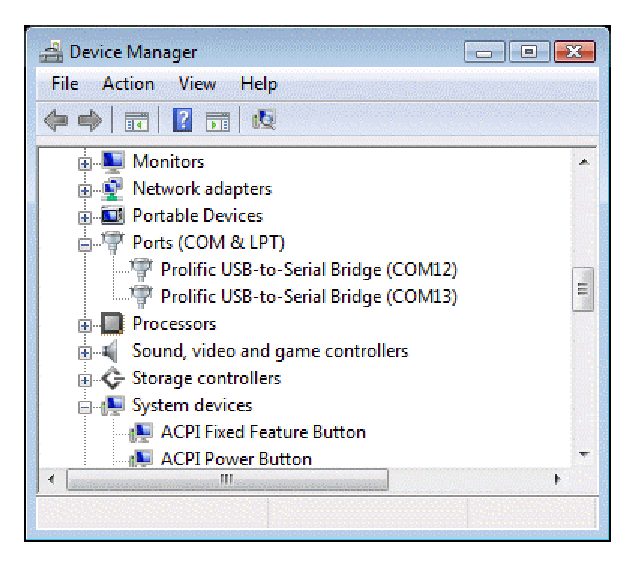
\includegraphics[width=4.6in]{devmancomassignmentsa.eps}
\caption{Screen Snapshot From \emph{Windows} Device Manager 
         (\emph{Windows Vista})}
\label{fig:susg0:sfdn0:01}
\end{figure}

Guessing the serial device names is not always possible, especially with USB adapters,
where the port numbers assigned may be $>10$ and may change when the USB adapter
is disconnected and reconnected to the computer.

The device names can typically be found by opening the \emph{Device Manager} (typically
under \emph{System} in the \emph{Windows} control panel).  (Naturally, the
devices must be plugged in if they are removable and the correct drivers
must be installed.)

Figure \ref{fig:susg0:sfdn0:01} is a screen snapshot from the \emph{Device Manager}
under \emph{Windows Vista}.  Under \emph{Ports (COM \& LPT)} it can be seen
in this figure that the device names are ``COM12'' and ``COM13''.


%%%%%%%%%%%%%%%%%%%%%%%%%%%%%%%%%%%%%%%%%%%%%%%%%%%%%%%%%%%%%%%%%%%%%%%%%%%%%%%
%%%%%%%%%%%%%%%%%%%%%%%%%%%%%%%%%%%%%%%%%%%%%%%%%%%%%%%%%%%%%%%%%%%%%%%%%%%%%%%
%%%%%%%%%%%%%%%%%%%%%%%%%%%%%%%%%%%%%%%%%%%%%%%%%%%%%%%%%%%%%%%%%%%%%%%%%%%%%%%
\subsection{Testing and Troubleshooting Serial Ports}
\label{susg0:stts0}

For testing and troubleshooting, it was found that
\index{Realterm@\emph{RealTerm}}\emph{RealTerm} \cite{bibref:swp:realterm}
(free open-source software) works very well for displaying the
characters received by a serial port.  
\index{Realterm@\emph{RealTerm}}\emph{RealTerm} is able to display all
received characters in hexadecimal, which is very helpful.

\begin{figure}
\centering
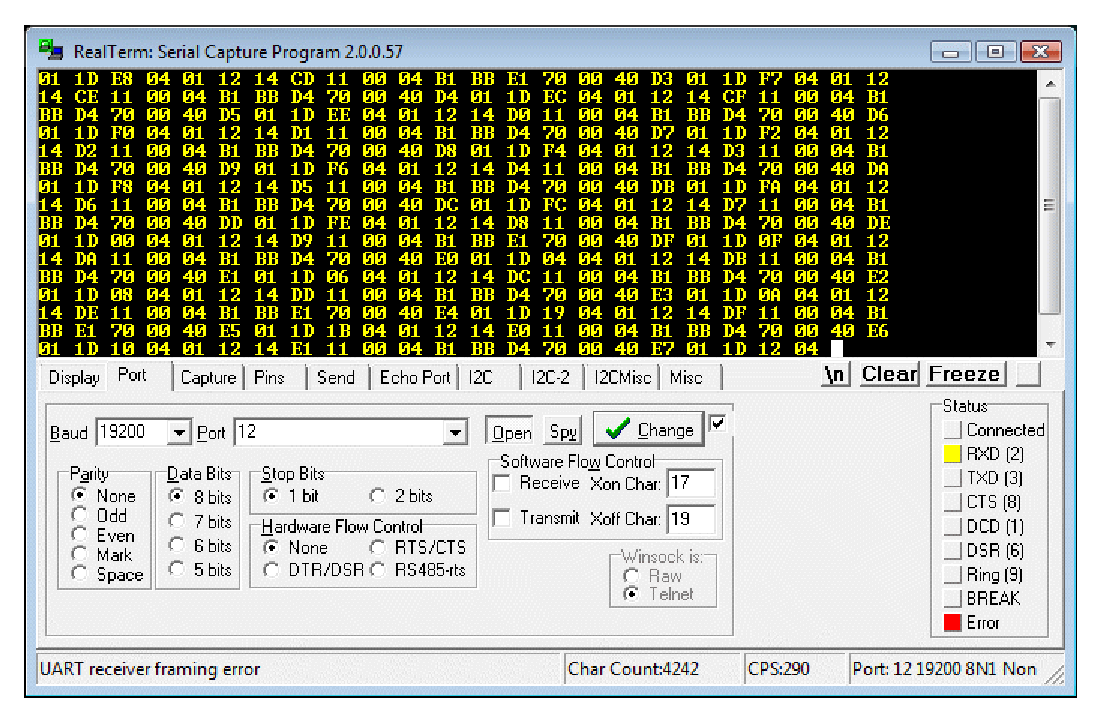
\includegraphics[width=4.6in]{rtermsnapshot01.eps}
\caption{\emph{RealTerm} Screen Snapshot (Hexadecimal Display Selected)}
\label{fig:susg0:stts0:01}
\end{figure}

Figure \ref{fig:susg0:stts0:01} is a screen snapshot of
\index{Realterm@\emph{RealTerm}}\emph{RealTerm} being used
to capture data.

\index{HyperTerminal@\emph{HyperTerminal}}\emph{HyperTerminal} (the default
serial communcation program in many versions of \emph{Windows})
is not recommended because of bugs involving bit 7 of incoming characters
(and perhaps other bugs as well).


%%%%%%%%%%%%%%%%%%%%%%%%%%%%%%%%%%%%%%%%%%%%%%%%%%%%%%%%%%%%%%%%%%%%%%%%%%%%%%%
%%%%%%%%%%%%%%%%%%%%%%%%%%%%%%%%%%%%%%%%%%%%%%%%%%%%%%%%%%%%%%%%%%%%%%%%%%%%%%%
%%%%%%%%%%%%%%%%%%%%%%%%%%%%%%%%%%%%%%%%%%%%%%%%%%%%%%%%%%%%%%%%%%%%%%%%%%%%%%%
\subsection{Program Invocation and Command-Line Parameters}
\label{susg0:spin0}

\productnameemph{} is typically invoked by opening a DOS shell and 
typing ``\texttt{\productname{}} \emph{ch0commport}
\emph{ch1commport} \emph{logcharstocon} \emph{logpacketstocon}'' (where
the four required parameters are described in detail below), 
followed by \emph{ENTER}.  Because the program creates the log files 
(\S{}\ref{susg0:slgf0}) in the current working directory, the desired
working directory is normally selected before invoking the program.

It is likely possible to invoke the program via the \emph{Windows} GUI,
but this has not been explored.

\productnameemph{} requires the following four command-line parameters:

\begin{itemize}
\item \emph{ch0commport}\\
      \emph{ch1commport}\\
      These two parameters are the serial port names
      of the communication ports to be used.
      
      By convention, Channel 0 (\emph{ch0commport} above) is the serial communication
      from the host microcontroller to the RF module, and Channel 1
      (\emph{ch1commport} above) is the
      serial communication from the RF module to the host microcontroller.

      For example, with the communication hardware implied by 
      Figure \ref{fig:susg0:sfdn0:01}, invoking the program using the
      command line\\\\
      \texttt{\productname{} com12 com13 n n}\\\\
      would result in the program expecting to listen to the output from
      the host microcontroller on \emph{com12} and the output from the
      RF module on \emph{com13}.
\item \emph{logcharstocon}\\
      \emph{logpacketstocon}\\
      Whether to log received characters and received packets, respectively,
      to the console (in addition to logging them to the
      character and packet log files).  

      The normal guesses for \emph{yes} and \emph{no}
      (``y'', ``1'', ``n'', ``0'', etc.) are all accepted.

      Errors are \emph{always} displayed on the console (as well as written to
      the alert log
      file).
\end{itemize}


%%%%%%%%%%%%%%%%%%%%%%%%%%%%%%%%%%%%%%%%%%%%%%%%%%%%%%%%%%%%%%%%%%%%%%%%%%%%%%%
%%%%%%%%%%%%%%%%%%%%%%%%%%%%%%%%%%%%%%%%%%%%%%%%%%%%%%%%%%%%%%%%%%%%%%%%%%%%%%%
%%%%%%%%%%%%%%%%%%%%%%%%%%%%%%%%%%%%%%%%%%%%%%%%%%%%%%%%%%%%%%%%%%%%%%%%%%%%%%%
\subsection{Program Termination}
\label{susg0:sptm0}

The \productnameemph{} program can be terminated by using CTRL-C.  Using 
CTRL-C once will signal the program to terminate the communication threads
in an orderly way, write trailing information to log files, and terminate.
Termination may take up to approximately 5 seconds.

The program will also terminate upon a variety of abnormal conditions,
such as unexpected errors from \emph{Win32} API functions.


%%%%%%%%%%%%%%%%%%%%%%%%%%%%%%%%%%%%%%%%%%%%%%%%%%%%%%%%%%%%%%%%%%%%%%%%%%%%%%%
%%%%%%%%%%%%%%%%%%%%%%%%%%%%%%%%%%%%%%%%%%%%%%%%%%%%%%%%%%%%%%%%%%%%%%%%%%%%%%%
%%%%%%%%%%%%%%%%%%%%%%%%%%%%%%%%%%%%%%%%%%%%%%%%%%%%%%%%%%%%%%%%%%%%%%%%%%%%%%%
\subsection{Log Files}
\label{susg0:slgf0}

When started, the \productnameemph{} program creates several log files in
the current working directory.  All of the created log files are 
plain text and can be viewed, manipulated, and printed
using a text editor.  This section describes these files.


%%%%%%%%%%%%%%%%%%%%%%%%%%%%%%%%%%%%%%%%%%%%%%%%%%%%%%%%%%%%%%%%%%%%%%%%%%%%%%%
%%%%%%%%%%%%%%%%%%%%%%%%%%%%%%%%%%%%%%%%%%%%%%%%%%%%%%%%%%%%%%%%%%%%%%%%%%%%%%%
%%%%%%%%%%%%%%%%%%%%%%%%%%%%%%%%%%%%%%%%%%%%%%%%%%%%%%%%%%%%%%%%%%%%%%%%%%%%%%%
\subsubsection{Log File Creation, Naming, and Syntax}
\label{susg0:slgf0:sfcn0}

Log files are named based on the local date and time in
YYYYMMDD\_HHMMSS format.   For example, a log file named
``\texttt{20090116\_131247\_alert.txt}'' was created at 
approximately 1:12 p.m. on January 16, 2009 (local time).

When started, \productnameemph{} creates an alert log file (containing error
messages), a character log file (containing a log of received characters,
serial events, and serial errors), a packet log file (containing 
information about parsed packets), and a comprehensive log file
(containing all log entries to any file).

Additionally, messages are written to the console (\S{}\ref{susg0:spin0}).

The naming convention for log files means that \productnameemph{}
can be run repeatedly in the same directory and the log file names will
not conflict.

A typical set of log file names from a single invocation of
\productnameemph{} is:

\begin{verbatim}
20090116_131247_alert.txt
20090116_131247_character.txt
20090116_131247_comprehensive.txt
20090116_131247_packet.txt
\end{verbatim}

Within each log file, entries are timestamped in HHMMSS.FFF format,
where ``FFF'' is the fractional portion of the second.


%%%%%%%%%%%%%%%%%%%%%%%%%%%%%%%%%%%%%%%%%%%%%%%%%%%%%%%%%%%%%%%%%%%%%%%%%%%%%%%
%%%%%%%%%%%%%%%%%%%%%%%%%%%%%%%%%%%%%%%%%%%%%%%%%%%%%%%%%%%%%%%%%%%%%%%%%%%%%%%
%%%%%%%%%%%%%%%%%%%%%%%%%%%%%%%%%%%%%%%%%%%%%%%%%%%%%%%%%%%%%%%%%%%%%%%%%%%%%%%
\subsubsection{Alert Log File Contents}
\label{susg0:slgf0:salf0}

The alert log file contains entries that indicate some sort of 
unusual event or logical problem.  The purpose of the alert log
file is to segregate error messages so that the other log files
do not have to be searched for error messages.  Generally, an
empty alert log file indicates no problems in SCI communication.

Typical entries from the alert log file are:

\begin{small}
\begin{verbatim}
131247.848:ALRT: CH01:Non-packet start event discarded: Character: 0x57.
131247.848:ALRT: CH01:Non-packet start event discarded: Character: 0xFF.
\end{verbatim}
\end{small}

Note that:

\begin{itemize}
\item All alert messages are also duplicated to the console.
\item Alert messages are usually also duplicated to the log files(s) 
      where the messages have relevance.  For example, the packet parse errors
      reproduced above would also be placed in the packet log file.
\end{itemize}


%%%%%%%%%%%%%%%%%%%%%%%%%%%%%%%%%%%%%%%%%%%%%%%%%%%%%%%%%%%%%%%%%%%%%%%%%%%%%%%
%%%%%%%%%%%%%%%%%%%%%%%%%%%%%%%%%%%%%%%%%%%%%%%%%%%%%%%%%%%%%%%%%%%%%%%%%%%%%%%
%%%%%%%%%%%%%%%%%%%%%%%%%%%%%%%%%%%%%%%%%%%%%%%%%%%%%%%%%%%%%%%%%%%%%%%%%%%%%%%
\subsubsection{Character Log File Contents}
\label{susg0:slgf0:sclf0}

The character log file contains a complete log of received characters,
serial events, and serial errors.

Typical entries from the character log file are:

\begin{footnotesize}
\begin{verbatim}
131247.848:NORM: CH00:<01><12><14><3A><11><00><04><B1><BB><D4><60><00><40><40>
131247.848:NORM: CH00:<01><1D><B4><04>
131247.879:NORM: CH00:<01><12><14><3B><11><00><04><B1><BB><D4><60>
131247.848:NORM: CH01:<57><FF><01><08><94><3A><01><00><D8><04>
131247.864:NORM: CH01:<01><15><95><41><11><D4><00><16><E6><04><B1><AA><EE><02>
131247.864:NORM: CH01:<01>
\end{verbatim}
\end{footnotesize}

Note in the text above
that the log entries between channels are slightly out of chronological order.
Please see \S{}\ref{skli0:sooc0}.


%%%%%%%%%%%%%%%%%%%%%%%%%%%%%%%%%%%%%%%%%%%%%%%%%%%%%%%%%%%%%%%%%%%%%%%%%%%%%%%
%%%%%%%%%%%%%%%%%%%%%%%%%%%%%%%%%%%%%%%%%%%%%%%%%%%%%%%%%%%%%%%%%%%%%%%%%%%%%%%
%%%%%%%%%%%%%%%%%%%%%%%%%%%%%%%%%%%%%%%%%%%%%%%%%%%%%%%%%%%%%%%%%%%%%%%%%%%%%%%
\subsubsection{Packet Log File Contents}
\label{susg0:slgf0:splf0}

The packet log file contains the parsed packets from the two communication channels.

Typical entries from the packet log file are:

\begin{footnotesize}
\begin{verbatim}
131455.144:NORM: CH01:ACK_SEND_DATA (0x94).
131455.144:NORM:      cspan=16, mdelta=109.
131455.144:NORM:      <01><08><94>
131455.144:NORM:      <6D><01><00>
131455.144:NORM:      <0B><04>
131455.144:NORM:      PACKET_ID: 0x6D, ACK_NACK: 0x01, NUM_RETRIES: 0x00.
131455.129:NORM: CH00:SEND_DATA (0x14).
131455.129:NORM:      cspan=15, mdelta=110.
131455.129:NORM:      <01><12><14>
131455.129:NORM:      <6D><11><00><04><B1><BB><D4><70><00><40><73><01><1D>
131455.129:NORM:      <2A><04>
131455.129:NORM:      PACKET_ID: 0x6D, TARGET_SENDER: 0x11, ADDRESS_MODE: 0x00.
131455.129:NORM:      DST_TRANS_AD: 0xB104.
131455.129:NORM:      DATA:
131455.129:NORM:      <BB><D4><70><00><40><73><01><1D>
131455.238:NORM: CH01:RXED_DATA (0x95).
131455.238:NORM:      cspan=15, mdelta=125.
131455.238:NORM:      <01><15><95>
131455.238:NORM:      <74><11><E4><00><16><E6><04><B1><AA><E7><02><01><80><6D>
131455.238:NORM:      <7E><FF>
131455.238:NORM:      <C3><04>
131455.238:NORM:      PACKET_ID: 0x74, TARGET_SENDER: 0x11, LQI: 0xE4.
131455.238:NORM:      ADDRESS_MODE: 0x00.
131455.238:NORM:      DST_TRANS_AD: 0xE616, SRC_TRANS_AD: 0xB104.
131455.238:NORM:      DATA:
131455.238:NORM:      <AA><E7><02><01><80><6D><7E><FF>
\end{verbatim}
\end{footnotesize}

Each parsed packet is documented as:

\begin{itemize}
\item The channel and packet type.
\item The approximate time span between the first and last 
      characters of the packet, in milliseconds (``\emph{cspan}'').
      A large value of \emph{cspan} would indicate some sort of
      a software error in transmitting the packet.
\item The approximate time since the last packet of this type
      was received (``\emph{mdelta}'').
\item The raw bytes of the packet, grouped by header, payload,
      and trailer.
\item The extracted data (symbolically) from the packet.
\end{itemize}

Note in the text above that the packet entries are sometimes
chronologically out of order between the two channels
(see \S{}\ref{skli0:soop0}).


%%%%%%%%%%%%%%%%%%%%%%%%%%%%%%%%%%%%%%%%%%%%%%%%%%%%%%%%%%%%%%%%%%%%%%%%%%%%%%%
%%%%%%%%%%%%%%%%%%%%%%%%%%%%%%%%%%%%%%%%%%%%%%%%%%%%%%%%%%%%%%%%%%%%%%%%%%%%%%%
%%%%%%%%%%%%%%%%%%%%%%%%%%%%%%%%%%%%%%%%%%%%%%%%%%%%%%%%%%%%%%%%%%%%%%%%%%%%%%%
\subsubsection{Comprehensive Log File Contents}
\label{susg0:slgf0:shlf0}

Each entry written to any other log file is also written to the
comprehensive log.  The comprehensive log is simply an interleaved concatenation
of the alert, character, and packet log files.


%%%%%%%%%%%%%%%%%%%%%%%%%%%%%%%%%%%%%%%%%%%%%%%%%%%%%%%%%%%%%%%%%%%%%%%%%%%%%%%
%%%%%%%%%%%%%%%%%%%%%%%%%%%%%%%%%%%%%%%%%%%%%%%%%%%%%%%%%%%%%%%%%%%%%%%%%%%%%%%
%%%%%%%%%%%%%%%%%%%%%%%%%%%%%%%%%%%%%%%%%%%%%%%%%%%%%%%%%%%%%%%%%%%%%%%%%%%%%%%
\subsubsection{Concurrent Access to Log Files Using a Text Editor}
\label{susg0:slgf0:scat0}

As the \productnameemph{} program may run for days or weeks at a time,
it is useful to examine the log files (especially the alert log) before
the program has terminated.

\productnameemph{} opens the log files in a mode compatible with sharing,
so they can be safely viewed read-only with a text editor while the program
is running.

Please see \S{}\ref{skli0:sndf0}.


%%%%%%%%%%%%%%%%%%%%%%%%%%%%%%%%%%%%%%%%%%%%%%%%%%%%%%%%%%%%%%%%%%%%%%%%%%%%%%%
%%%%%%%%%%%%%%%%%%%%%%%%%%%%%%%%%%%%%%%%%%%%%%%%%%%%%%%%%%%%%%%%%%%%%%%%%%%%%%%
%%%%%%%%%%%%%%%%%%%%%%%%%%%%%%%%%%%%%%%%%%%%%%%%%%%%%%%%%%%%%%%%%%%%%%%%%%%%%%%
\section{Known Issues and Limitations}
\label{skli0}

This section describes known issues and limitations with the
\productnameemph{} program or the hardware configuration
described in \S{}\ref{shsu0:sdph0}.


%%%%%%%%%%%%%%%%%%%%%%%%%%%%%%%%%%%%%%%%%%%%%%%%%%%%%%%%%%%%%%%%%%%%%%%%%%%%%%%
%%%%%%%%%%%%%%%%%%%%%%%%%%%%%%%%%%%%%%%%%%%%%%%%%%%%%%%%%%%%%%%%%%%%%%%%%%%%%%%
%%%%%%%%%%%%%%%%%%%%%%%%%%%%%%%%%%%%%%%%%%%%%%%%%%%%%%%%%%%%%%%%%%%%%%%%%%%%%%%
\subsection{Possible Destruction of the ADM3232 Part}
\label{skli0:sdap0}

The level conversion board used is designed to be powered from the same power supply
as the microcontroller.

It is suspected that as the batteries discharge, the TTL 
SCI inputs from a product may
damage the \index{ADM3232}ADM3232 part (as the 
inputs may be more than a diode drop above the
supply voltage provided by the batteries).

In retrospect, rather than using 3 AA 
batteries in series (4.5 volts),
it would have been more prudent to use 
4 AA batteries in series (6.0 volts) 
with a forward-biased diode to bring the supply 
voltage down to about 5.4 volts.

A resistor in series with the SCI inputs 
(not included in the first version
of the SCI interface box) may also be prudent.


%%%%%%%%%%%%%%%%%%%%%%%%%%%%%%%%%%%%%%%%%%%%%%%%%%%%%%%%%%%%%%%%%%%%%%%%%%%%%%%
%%%%%%%%%%%%%%%%%%%%%%%%%%%%%%%%%%%%%%%%%%%%%%%%%%%%%%%%%%%%%%%%%%%%%%%%%%%%%%%
%%%%%%%%%%%%%%%%%%%%%%%%%%%%%%%%%%%%%%%%%%%%%%%%%%%%%%%%%%%%%%%%%%%%%%%%%%%%%%%
\subsection{Ground Offset Issues}
\label{skli0:sgoi0}

It was observed that the hardware interface box
(\S{}\ref{shsu0:sdph0}, p. \pageref{shsu0:sdph0})
works perfectly when using a laptop computer, but 
less reliably when using a desktop computer.

When the interface box fails to operate, the problem can usually
be cured by disconnecting and then reconnecting the serial cables
to the PC and/or the SCI connections to the microcontroller product.

A ground offset issue involving the power supply and the PC 
is suspected.


%%%%%%%%%%%%%%%%%%%%%%%%%%%%%%%%%%%%%%%%%%%%%%%%%%%%%%%%%%%%%%%%%%%%%%%%%%%%%%%
%%%%%%%%%%%%%%%%%%%%%%%%%%%%%%%%%%%%%%%%%%%%%%%%%%%%%%%%%%%%%%%%%%%%%%%%%%%%%%%
%%%%%%%%%%%%%%%%%%%%%%%%%%%%%%%%%%%%%%%%%%%%%%%%%%%%%%%%%%%%%%%%%%%%%%%%%%%%%%%
\subsection{Startup Difficulties}
\label{skli0:ssud0}

The \productnameemph{} may not start reliably in the presence of serial
errors or events (such as a break event on the serial line, typically
caused by the target module being turned off but the interface box being turned
on).  
A typical error message involves inability to 
obtain serial port state or configure the port.

To get \productnameemph{} to start, remove the serial error, start the
program, then reapply the source of the errors.  The two easiest approaches
are:

\begin{itemize}
\item Disconnect the serial cables from the serial adapters, start the program,
      then reconnect the cables.
\item Turn off the interface box, start the program, then turn on the interface box.
\item Power up everything (including the target product) before starting the
      program.
\end{itemize} 

The root cause is that the serial errors cause (by design) certain 
\emph{Windows} API functions not to operate until the error is cleared using
another \emph{Windows} API function.  The present version of the program will
correctly handle serial errors at any time except startup.

This is a very minor issue and does not affect the logical correctness
of the program once it is running.


%%%%%%%%%%%%%%%%%%%%%%%%%%%%%%%%%%%%%%%%%%%%%%%%%%%%%%%%%%%%%%%%%%%%%%%%%%%%%%%
%%%%%%%%%%%%%%%%%%%%%%%%%%%%%%%%%%%%%%%%%%%%%%%%%%%%%%%%%%%%%%%%%%%%%%%%%%%%%%%
%%%%%%%%%%%%%%%%%%%%%%%%%%%%%%%%%%%%%%%%%%%%%%%%%%%%%%%%%%%%%%%%%%%%%%%%%%%%%%%
\subsection{Inability to Determine Timing Relationships Between Channels}
\label{skli0:itr0}

The three-thread software design may lead to more timestamp inconsistency
between the two channels than necessary.  If possible, the design should probably
be changed to two threads and overlapped I/O.

The timestamps have, however, proved to be very accurate.


%%%%%%%%%%%%%%%%%%%%%%%%%%%%%%%%%%%%%%%%%%%%%%%%%%%%%%%%%%%%%%%%%%%%%%%%%%%%%%%
%%%%%%%%%%%%%%%%%%%%%%%%%%%%%%%%%%%%%%%%%%%%%%%%%%%%%%%%%%%%%%%%%%%%%%%%%%%%%%%
%%%%%%%%%%%%%%%%%%%%%%%%%%%%%%%%%%%%%%%%%%%%%%%%%%%%%%%%%%%%%%%%%%%%%%%%%%%%%%%
\subsection{Out-of-Order Character Logging}
\label{skli0:sooc0}

The primary thread dequeues and processes all characters from 
Channel 0, then dequeues and processes all characters from Channel 1;
regardless of the chronological ordering of the characters between the
channels.
This can result in characters being logged out of chronological order if
characters are arriving on both channels nearly simultaneously.

This problem can be easily fixed by changing the character logging
algorithm to dequeue the characters in chronological order with respect
to
both queues.

This problem does not affect the correctness of the timestamps in the 
character log file.  It only affects the ordering of the log
entries.  Please see the sample log file text in
\S{}\ref{susg0:slgf0:sclf0}, p. \pageref{susg0:slgf0:sclf0}.


%%%%%%%%%%%%%%%%%%%%%%%%%%%%%%%%%%%%%%%%%%%%%%%%%%%%%%%%%%%%%%%%%%%%%%%%%%%%%%%
%%%%%%%%%%%%%%%%%%%%%%%%%%%%%%%%%%%%%%%%%%%%%%%%%%%%%%%%%%%%%%%%%%%%%%%%%%%%%%%
%%%%%%%%%%%%%%%%%%%%%%%%%%%%%%%%%%%%%%%%%%%%%%%%%%%%%%%%%%%%%%%%%%%%%%%%%%%%%%%
\subsection{Out-of-Order Packet Logging}
\label{skli0:soop0}

The packet logging issue occurs for exactly the same reasons as the
character logging issue discussed in 
\S{}\ref{skli0:sooc0}.  The solution is analogous---to modify the
packet logging algorithm to process both queues simultaneously and
log packets in chronological order.

The sample text in \S{}\ref{susg0:slgf0:splf0}, p. \pageref{susg0:slgf0:splf0}
illustrates the issue.  The SEND\_DATA packet is sent at 131455.129 and it is
followed by the ACK\_SEND\_DATA packet at 131455.144; but the log entries are 
not in chronological order.

This issue does not affect the correctness of the log entries---only their 
ordering.


%%%%%%%%%%%%%%%%%%%%%%%%%%%%%%%%%%%%%%%%%%%%%%%%%%%%%%%%%%%%%%%%%%%%%%%%%%%%%%%
%%%%%%%%%%%%%%%%%%%%%%%%%%%%%%%%%%%%%%%%%%%%%%%%%%%%%%%%%%%%%%%%%%%%%%%%%%%%%%%
%%%%%%%%%%%%%%%%%%%%%%%%%%%%%%%%%%%%%%%%%%%%%%%%%%%%%%%%%%%%%%%%%%%%%%%%%%%%%%%
\subsection{Suspected Out of Sequence Communication Errors}
\label{skli0:sose0}

It is suspected that framing errors and other errors become events
that are reported out of sequence by the communication worker threads.
The root cause is that communication errors may occur with characters 
buffered behind the \emph{Windows} API.

The \productnameemph{} program handles errors first, then dequeues any characters;
although the characters probably came first, followed by the error.

The problem can be fixed by experimenting to determine the behavior of
\emph{Windows} and then changing the communication worker threads to match.

This issue is inconsequential because any communication error
(break, framing error, overrun, etc.) is very serious if it occurs
once the target product is operating, and exactly when it occurred is
less important than that it did occur.

The errors will be detected,
but they may
be slightly out of sequence in the event queue.


%%%%%%%%%%%%%%%%%%%%%%%%%%%%%%%%%%%%%%%%%%%%%%%%%%%%%%%%%%%%%%%%%%%%%%%%%%%%%%%
%%%%%%%%%%%%%%%%%%%%%%%%%%%%%%%%%%%%%%%%%%%%%%%%%%%%%%%%%%%%%%%%%%%%%%%%%%%%%%%
%%%%%%%%%%%%%%%%%%%%%%%%%%%%%%%%%%%%%%%%%%%%%%%%%%%%%%%%%%%%%%%%%%%%%%%%%%%%%%%
\subsection{Non-Detection of Log File Flushes}
\label{skli0:sndf0}

\productnameemph{} flushes the log file streams every 15 seconds using
the \emph{fflush()} function.  Still, 
\index{SlickEdit@\emph{SlickEdit}}\emph{SlickEdit}
(the text editor I use) does not
exhibit the desired behavior of detecting the updated file when focus
is restored.  In order to see additions to a log file, the file must be
closed and then re-opened in \emph{SlickEdit}.

The technical basis for this non-detection should be investigated.

Note that this limitation does not affect the correctness or completeness
of any log file---it only affects whether a typical text editor will
automatically detect that the open file has changed.


%%%%%%%%%%%%%%%%%%%%%%%%%%%%%%%%%%%%%%%%%%%%%%%%%%%%%%%%%%%%%%%%%%%%%%%%%%%%%%%

%\clearpage{}
%\section{Glossary of Terms, Acronyms, and Nomenclature}
%\label{sglo1}

%\begin{docglossaryenum}

%\item \index{fTq@$f_{T_q}$}$f_{T_q}$

%      \cite[p. 161]{bibref:freescale:gz60a} defines $f_{T_q}$ as the
%      frequency of $T_q$, the atomic unit of time handled by the HSCAN
%      peripheral built in to the microcontroller.

%\end{docglossaryenum}

%%%%%%%%%%%%%%%%%%%%%%%%%%%%%%%%%%%%%%%%%%%%%%%%%%%%%%%%%%%%%%%%%%%%%%%%%%%%%%%
\clearpage{}
\addcontentsline{toc}{section}{References}

\begin{thebibliography}{000}
\bibitem{bibref:vendor:dynex}
   \emph{Dynex},\\
   \texttt{http://www.dynexproducts.com}
\bibitem{bibref:vendor:futurelec}
   \emph{Futurelec},\\
   \texttt{http://www.futurelec.com}
\bibitem{bibref:twp:ms810467}
   \emph{Serial Communications in Win32},\\
   \texttt{http://msdn.microsoft.com/en-us/library/ms810467.aspx}
\bibitem{bibref:swlic:gpl}
   \emph{GNU General Public License},\\
   \texttt{http://www.gnu.org/licenses/licenses.html}
\bibitem{bibref:osws:sourceforge}
   \emph{SourceForge},\\
   \texttt{http://www.sourceforge.net}
\bibitem{bibref:i:daveashley}
   David T. Ashley,\\
   \texttt{dashley@gmail.com}
\bibitem{bibref:swp:slickedit}
   \emph{SlickEdit},\\
   \texttt{http://www.slickedit.com}
\bibitem{bibref:swp:realterm}
   \index{Realterm@\emph{RealTerm}}\emph{RealTerm},\\
   \texttt{http://realterm.sourceforge.net}
\end{thebibliography}

%%%%%%%%%%%%%%%%%%%%%%%%%%%%%%%%%%%%%%%%%%%%%%%%%%%%%%%%%%%%%%%%%%%%%%%%%%%%%%%
\clearpage{}
\addcontentsline{toc}{section}{Index}
\printindex

%%%%%%%%%%%%%%%%%%%%%%%%%%%%%%%%%%%%%%%%%%%%%%%%%%%%%%%%%%%%%%%%%%%%%%%%%%%%%%%
\end{document}
%
%$Log: man20081211a.tex,v $
%Revision 1.20  2009/01/17 22:17:01  dashley
%Edits.
%
%Revision 1.19  2009/01/17 20:08:12  dashley
%Edits.
%
%Revision 1.18  2009/01/17 05:25:40  dashley
%Edits.
%
%Revision 1.17  2009/01/17 04:28:05  dashley
%Edits.
%
%Revision 1.16  2009/01/17 01:09:00  dashley
%Edits.
%
%Revision 1.15  2009/01/16 21:32:38  dashley
%Edits.
%
%End of $RCSfile: man20081211a.tex,v $.
%%%%%%%%%%%%%%%%%%%%%%%%%%%%%%%%%%%%%%%%%%%%%%%%%%%%%%%%%%%%%%%%%%%%%%%%%%%%%%%
